% SPDX-License-Identifier: LPPL-1.3c
% Copyright (C) 2026 Christophe Jorssen
% Author and Current Maintainer: Christophe Jorssen <christophe.jorssen@gmail.com>
% LPPL maintenance status: maintained
% This file is part of luafemm. See LICENSE and LICENSES.md for its terms.
\section{Exchanging electrostatic problems with FEMM}
\label{sec:electric-exchange}

A native |.fee| file describes a two-dimensional electrostatic problem. A native
|.res| file adds its triangular mesh and nodal potentials. Both FEMM~4 and FEMM~5
use electrostatic format~1; their common extension does not identify the solver
edition. The library reads these files as data, never as executable Lua or TeX.
No FEMM executable, native library or shell escape is required by the package.
Unknown physical records and missing volume-charge density fields are rejected;
the adapter does not guess a different material law.

Importing a problem rebuilds its mesh and solves it in Lua. Importing an answer
preserves its mesh and potentials: drawing a field or capturing a profile does
not replace the imported solution by another solve. Fields are raw P1 gradients,
without FEMM's optional smoothing. A capacitance matrix, in contrast, deliberately
solves its independent excitation problems on that mesh.

\subsection{A complete export and restoration}
\luafemmexamplebegin{electric-exchange}
Start with a coarse mesh. Declare the physical paths before the first field,
profile, matrix, force or export request. Exporting |fee| constructs the mesh;
exporting |res| also solves the problem. A named picture keeps an owned solution
for later exports, just as it does for profiles and matrices.

\Needspace{12cm}
\begin{codeexample}[width=0pt]
\begin{tikzpicture}[femm/electrostatic={model=finite elements,
 xmin=0,xmax=2,ymin=0,ymax=1,outer boundary=insulated,
 mesh size=.35,name=exchange cell},scale=2]
 \draw[very thick,femm/electric electrode={name=left,potential=10}]
   (0,0)--(0,1);
 \draw[very thick,femm/electric electrode={name=right,potential=0}]
   (2,0)--(2,1);
 \draw[orange!80!black,thick,
   femm/electric electrode={name=screen,condition=charge}]
   (1,.25)--(1,.75);
 \pic {femm electric field};\pic {femm equipotentials};
\end{tikzpicture}
\femmelectricexport[model=exchange cell,
 file=\jobname-electric.fee,edition=femm5]
\femmelectricexport[model=exchange cell,
 file=\jobname-electric.res,format=res,edition=femm5]
\end{codeexample}

The exported files use metres internally. Choosing |length unit=cm| when
importing expresses their coordinates in centimetres for TikZ, without changing
the physical problem. This is the default model unit. Canvas scaling and rotation
remain ordinary TikZ operations. The file supplies its physical domain bounds,
materials, sources, conductors and reference potential; do not redeclare them.

\Needspace{10cm}
\begin{codeexample}[width=0pt]
\begin{tikzpicture}[femm/electrostatic={
 file=\jobname-electric.res,file edition=femm5},scale=2]
 \pic {femm electric geometry};
 \pic {femm electric field};
 \path[femm/electric profile={name=restored potential,samples=41}]
   (.05,.5)--(1.95,.5);
\end{tikzpicture}
\end{codeexample}

The field and the following curve use the same stored nodal solution. A profile
through an excluded conductor interior instead needs |outside=nan| to show the
gap. The thin screen here has no excluded interior.

\Needspace{10cm}
\begin{codeexample}[width=0pt]
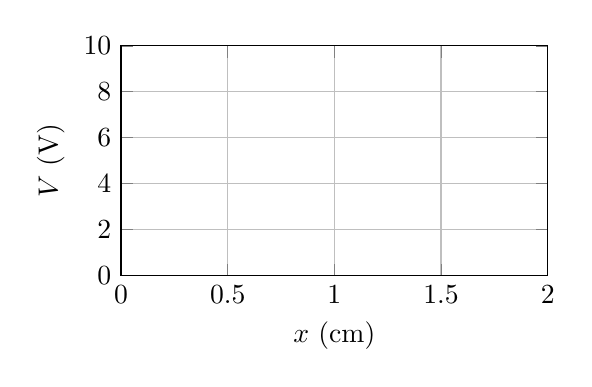
\begin{tikzpicture}
 \begin{axis}[width=7cm,height=4.5cm,
   xlabel={$x$ (cm)},ylabel={$V$ (V)},grid=major,
   xmin=0,xmax=2,ymin=0,ymax=10]
  \femmelectricplot[profile=restored potential,
    component=V,abscissa=x,plot options={blue,thick,mark=none}]
 \end{axis}
\end{tikzpicture}
\end{codeexample}

To recompute the exported problem, use |file=\jobname-electric.fee| instead.
The next view uses a requested global spacing of $2.5$~mm. This spacing is an
import control in metres, independent of the displayed coordinate unit.
It can add vertices inside the exported triangular cells, but cannot remove their
constrained edges. To obtain a coarser native geometry, export from a coarser
original mesh.

\begin{codeexample}[width=0pt]
\begin{tikzpicture}[femm/electrostatic={
 file=\jobname-electric.fee,file edition=femm5,
 import mesh size=.0025,import curve tolerance=.00001},scale=2]
 \pic {femm electric geometry};
 \pic[femm/electric={level count=8}] {femm equipotentials};
\end{tikzpicture}
\end{codeexample}
\luafemmexampleend{electric-exchange}

\subsection{Import keys and operation order}
\begin{key}{/femm/electrostatic/file=\meta{filename} (initially empty)}
  Picture-local native input. Empty means an ordinary model or snapshot.
  A nonempty input selects the FE provider and reads either problem or answer
  records by their contents. The filename is resolved through the format's file
  resolver, then the engine output directory for a preceding export.
  |file| and |snapshot| are mutually exclusive. Physical model overrides and
  subsequent physical path declarations are errors. Use ordinary TikZ paths
  for annotations and clipping, and the electric pics/profile keys for results.
\end{key}
\begin{key}{/femm/electrostatic/file edition=\meta{femm4 or femm5} (initially femm5)}
  Physical interpretation of the native data, local to the picture. Select
  |femm4| for FEMM~4 and xfemm. The edition cannot be inferred from format~1.
  It controls the internal surface-charge convention described below; it does
  not convert a three-dimensional model into a planar one.
\end{key}
\begin{key}{/femm/electrostatic/import mesh size=\meta{positive number} (initially empty)}
  Global target spacing in metres for problem import. When empty, use the
  smaller of one sixteenth of the largest domain span and positive native block
  label sizes or FEMM~5 point feature sizes. Native segment size limits remain
  constraints. An explicit value replaces that automatic global choice.
  The native minimum-angle and smart-mesh heuristics are not reproduced.
  This key does not refine a stored answer mesh.
\end{key}
\begin{key}{/femm/electrostatic/import curve tolerance=\meta{positive number} (initially .00001)}
  Maximum chord sagitta in metres for imported circular arcs in a problem.
  The native arc subdivision angle is also respected. Refine this tolerance
  together with the mesh for curved electrodes. For an answer, use the actual
  arc vertices already present in its mesh, without resampling the solution.
\end{key}

The existing |length unit| key selects the imported model-coordinate unit.
Input files may use inches, millimetres, centimetres, metres, mils or microns;
all physical lengths are converted before assembly. Planar depth is preserved
as a physical length. Axisymmetric coordinates are $r,z$, with full-revolution
charge and energy. Negative-radius geometry and external-region transforms fail.

The reliable sequence is: select the file and edition at picture start; draw
geometry or fields; capture measurements; use named snapshots outside the
picture. Reading a |fee| does not by itself solve it. The first evaluation, or
retaining a named snapshot at picture end, does. Once imported, the physical
model belongs to that file. A different excitation requires another input file
or an independently declared TikZ model.

\subsection{Export keys and representation}
\begin{command}{\femmelectricexport\opt{\oarg{options}}}
  Write a native electrostatic problem or answer using the keys below. With an
  empty |model|, use the current electric picture; otherwise use the named owned
  snapshot. Declare every physical path first. The destination's parent directory
  must exist. Relative output filenames follow the engine's output directory.
  All representation checks precede an atomic replacement of the output file.
  An imported source file cannot be overwritten, including through a filesystem
  alias. Use a distinct filename for a new export.
\end{command}
\begin{key}{/femm/electric export/file=\meta{filename} (initially empty)}
  Required destination, ending in |.fee| or |.res| consistently with |format|.
  Filename text is escaped across the TeX/Lua boundary.
\end{key}
\begin{key}{/femm/electric export/model=\meta{name} (initially empty)}
  Name of an electric snapshot; empty selects the current picture.
  Analytical Coulomb and symmetry providers cannot be exported natively.
\end{key}
\begin{key}{/femm/electric export/format=\meta{fee or res} (initially fee)}
  |fee| writes the computational problem. |res| adds the solved mesh, nodal
  potentials and conductor voltage/total-charge records. No native solver is
  invoked. Re-exporting an imported answer preserves its nodal solution.
\end{key}
\begin{key}{/femm/electric export/edition=\meta{femm4 or femm5} (initially femm5)}
  Target solver convention. Select |femm4| for xfemm as well as FEMM~4.
  Use the same edition on re-import. This changes the representation of internal
  prescribed sheet charge where needed, without changing the LuaFEMM model.
\end{key}

Export uses the actual computational polygonal geometry, including flattened
B\'ezier paths, overlapping material precedence and conductor boundaries. Each
active triangle becomes one labelled native cell, and solid conductor triangles
become holes. Auxiliary cell edges are marked hidden for the geometry view;
physical interfaces remain visible. This gives unambiguous material ownership and native solution-label
indices at the cost of a larger, triangulated CAD drawing. It is not a recovery
of the original TikZ source, nor a compact arc-fitting operation. The original
TikZ paths and their appearance remain unchanged.

Native dielectric records have only the coordinate-aligned components
$\epsilon_x,\epsilon_y$. A nonzero off-diagonal component is rejected, rather
than replaced by an isotropic average. Periodic problem import is limited to
straight translated pairs on opposite sides of the bounding rectangle, with the
same restrictions as Section~\ref{sec:electric-extended}. Periodic native answer
import and periodic native export are not supported. Rotational interfaces,
nonlinear/lossy dielectrics, arbitrary three-dimensional FE and native exterior
transformations are also outside this exchange contract.

\subsection{Native source semantics and numerical limits}
A native point property with |qp| in C/m contributes a transverse line source
in planar geometry, or a ring with $Q=2\pi r q_p$ in axisymmetry. Its radial
weight vanishes at $r=0$. If |qp=0|, the same native record instead prescribes
its point voltage |Vp|. Such point constraints are mesh-dependent idealizations;
a singular source's nodal potential is not a finite physical source potential.
Sampling exactly at an active nonzero source returns an invalid value. Validate
field/potential convergence away from the source, and prefer finite electrodes
for capacitance and force experiments. The analytical |femm/point charge| node
continues to mean a three-dimensional Coulomb charge in C and is never aliased
to these native records.

A fixed native voltage takes precedence over a coincident source load. Conflicting
voltages fail explicitly. A point charge assigned to a floating conductor is
rejected because its source/constraint precedence is not part of this contract.
Native voltage/conductor segments on the regular axis impose nodal constraints,
although their surface measure is zero; ordinary TikZ axis paths retain their
insulated-axis rules.

In the inspected FEMM~4/xfemm loader an internal |qs| distribution is assigned to
one adjacent element. In the inspected FEMM~5 loader it is assigned to both.
Thus |edition=femm5| writes half the total sheet density on an internal edge,
whereas |edition=femm4| writes the full density. Exterior surface charge has
only one adjacent element in either edition. The mixed convention is
$\mathbf D\cdot\mathbf n=c_0V+c_1$, with nonnegative $c_0$; it is supported on
exterior edges. An unspecified native exterior is naturally insulated.

Imported answers retain their raw nodal values. Energy, displacement and reaction
charges are evaluated with this library's P1 measures; axisymmetric source and
Robin quadratures need not equal native solver quadratures on a coarse mesh.
A solver residual is therefore not advertised for a stored native answer.
The original native conductor result records remain in its owned data, while
public charge measurements use the reconstructed variational reactions.
An imported answer is not a certificate of accuracy: compare mesh and arc
refinement, source distance and domain size for the physical quantity of interest.
